\section{Integração com Middleware \textit{uOS}}

	A integração do Middleware \textit{uOS} com o Sistema TRUE consiste em um \textit{driver} desenvolvido para que ambos possam se comunicar. Este \textit{driver} foi nomeado de \textit{UserDriver} que foi apresentado na Seção~\ref{sec:modulo-integracao}. Com intuito de exemplificar a utilização do \textit{UserDriver} e testar a integração do Sistema TRUE com o middleware \textit{uOS} foi desenvolvido uma aplicação para o middleware chamada \textit{UserApp}. Esta aplicação registra um \textit{listener} para ``escutar'' os eventos do \textit{UserDriver} chamado \textit{UserListener}. 

	Como aplicação o \textit{UserApp} apenas se inscreve para receber os eventos gerados pelo \textit{UserDriver}. Já o \textit{UserListener}, como \textit{listener}, espera os eventos serem gerados e realiza duas análises: analisa o evento (novo usuário detectado, usuário perdido, ou reconhecimento realizado) e analisa quanto tempo cada usuário está parado no mesmo lugar.

		% \begin{figure}[hbt]
		% 	\begin{center}
		% 		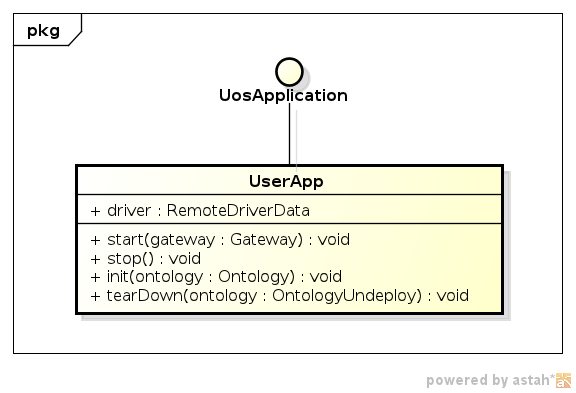
\includegraphics[scale=0.6]{figuras/5.Testes/diagrama-classe-user-ap.png}
		% 	\end{center}
		% 	\caption{Diagrama de Classe da aplicação \textit{UserApp}.}
		% 	\label{fig:diagrama-userapp}
		% \end{figure}

		% \begin{figure}[hbt]
		% 	\begin{center}
		% 		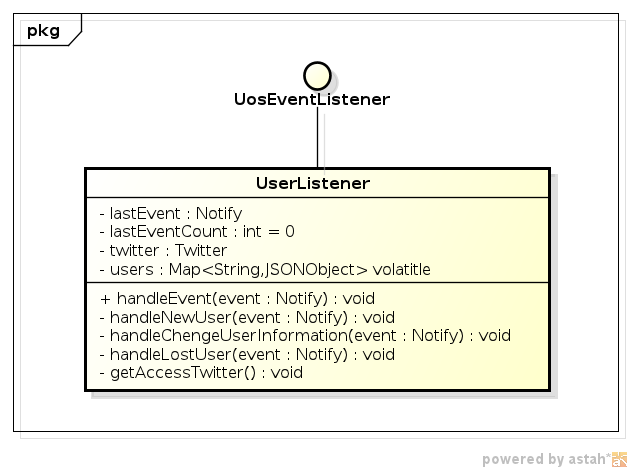
\includegraphics[scale=0.6]{figuras/5.Testes/diagrama-classe-user-listener.png}
		% 	\end{center}
		% 	\caption{Diagrama de Classe do \textit{listener} \textit{UserListener}.}
		% 	\label{fig:diagrama-userlistener}
		% \end{figure}

	% Basicamente, quando o \textit{UserListener} obtém os eventos do \textit{UserDriver}, ele envia mensagens pelo Twitter~\cite{twitter} para os usuários no ambiente, conforme o evento recebido. Para enviar as mensagens pelo Twitter foi utilizado a biblioteca \textit{twitter4j}~\cite{twitter4j}. A Figura~\ref{fig:diagrama-tweet} mostra o fluxo básico de execução do \textit{listener} e as mensagens padrões para cada tipo de evento recebido. 

	Basicamente, quando o \textit{UserListener} é inicializado ele obtém acesso ao twitter e se registra para escutar os eventos gerados pelo \textit{UserDriver}. Para cada evento obtido, ele envia mensagens pelo Twitter~\cite{twitter} para os usuários no ambiente. Para eventos de ``novo usuário detectado'' e ``usuário perdido'', ele envia mensagens de boas vindas e de despedidas respectivamente. Como mencionado na Seção~\ref{sec:modulo-integracao}, o \textit{UserDriver} também gera eventos de atualização dos dados dos usuários. Quando estes eventos são gerados, o \textit{UserListener} verifica se houve atualização na identidade do usuário e se o mesmo está a mais de uma hora no mesmo lugar. Caso esteja, ele envia mensagens aos usuários informando estes acontecimentos. Este fluxo de execução e as estruturas das mensagens enviadas são mostrados na Figura~\ref{fig:diagrama-tweet}. Para enviar as mensagens pelo Twitter foi utilizado a biblioteca \textit{twitter4j}~\cite{twitter4j}.

	\begin{figure}[hbt]
		\begin{center}
			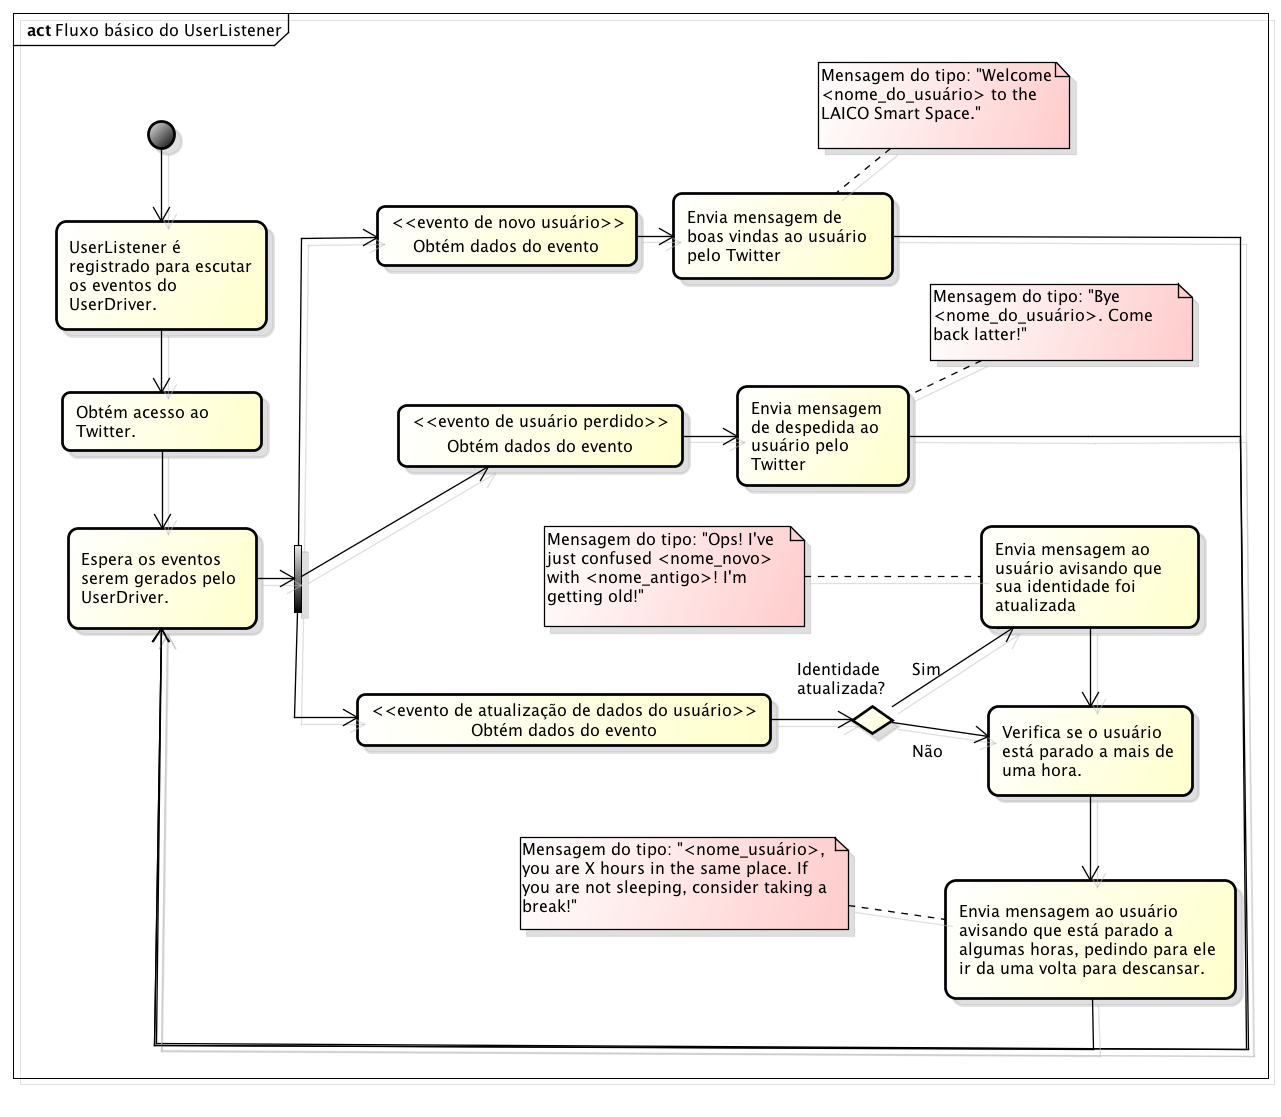
\includegraphics[scale=0.45]{figuras/5.Testes/diagrama-user-tweet.png}
		\end{center}
		\caption{Fluxo básico de execução do \textit{listener} \textit{UserListener}.}
		\label{fig:diagrama-tweet}
	\end{figure}

	Testes funcionais foram feitos com a aplicação mostrando que o \textit{driver} consegue
	obter os dados íntegros do Sistema TRUE e gerar os eventos de maneira praticamente
	instantânea. Algumas vezes as mensagens demoravam a chegar ao Twitter,
	geralmente nos horários de pico quando o Twitter operava próximo ao limite
	da sua capacidade. A Figura~\ref{fig:tweets} mostra as mensagens geradas
	pela aplicação em um teste funcional, onde Danilo, um usuário cadastrado,
	entra no ambiente senta em uma mesa com seu notebook permanecendo no mesmo
	lugar por mais de uma hora, e logo depois deixa o ambiente.

	\begin{figure}[hbt]
			\begin{center}
				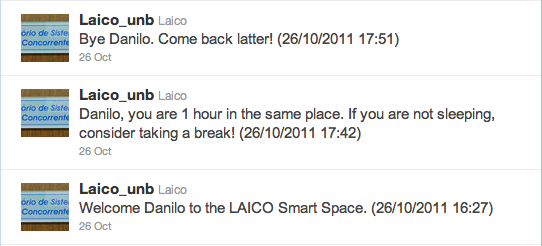
\includegraphics[scale=0.6]{figuras/5.Testes/tweets.png}
			\end{center}
			\caption{Exemplo das mensagens enviadas pelo Twitter aos usuários no ambiente.}
			\label{fig:tweets}
		\end{figure}	